%% 방법 논문 초판(v0.1)의 한국어 번역본(검토·공유용). 제출본은 영어 main.tex이다.
%% Overleaf: Main document = main_ko.tex, Compiler = pdfLaTeX (한글 글꼴 오류 시 XeLaTeX).
\documentclass[twocolumn,10pt]{article}
\usepackage[letterpaper,margin=0.75in,columnsep=0.25in]{geometry}
\usepackage{kotex}
\usepackage[round]{natbib}
\usepackage{graphicx}
\usepackage{amsmath}
\usepackage{amssymb}
\usepackage{booktabs}
\usepackage{xcolor}
\usepackage[small]{caption}
\usepackage{url}
\usepackage{algorithm}
\usepackage{algpseudocode}

\newcommand{\todo}[1]{\textcolor{red}{[TODO: #1]}}
\newcommand{\tbd}{\textcolor{red}{TBD}}
\newcommand{\pilot}{\textsuperscript{\textcolor{gray}{$\dagger$}}}
\newcommand{\sg}{\operatorname{sg}}
\newcommand{\JS}{\operatorname{JS}}
\newcommand{\ours}{PGCT}
\floatname{algorithm}{알고리즘}

\title{누구와 공유할지 학습하기:\\ 잠재 팀이 있는 다중 agent 강화학습을 위한 정책 gate 기반 critic 전이}
\author{익명 제출 (한국어 번역본)}
\date{}

\begin{document}
\maketitle

\begin{abstract}
목표가 서로 다른 여러 학습 agent 집단이 한 환경을 공유할 때, agent 사이의 지식 공유는 학습을 빠르게 할 수 있다.
하지만 올바른 agent끼리 공유할 때만 그렇고, 실제로는 팀 소속을 모르는 경우가 많다. 우리는 각 agent가 국소적
상호작용으로부터 누구의 가치 추정을 배울지 스스로 정하는 분산 방법인 정책 gate 기반 critic 전이(\ours{})를 제안한다.
이웃 agent들은 미리 합의한 고정 probe 관측 집합에서 행동 분포를 비교한다. 평활화한 Jensen--Shannon gate가 호환되는
상대를 고르고, agent는 그 상대의 critic을 probe 입력에서 distillation한다. actor와 자기 경험은 공유하지 않는다. 팀 라벨,
원시 관측, 파라미터는 교환하지 않는다. 처음부터 학습한 두 팀 다중 로봇 창고 과제의 예비 결과\todo{seed 1개; seed 2--$n$으로
갱신}에서, \ours{}는 독립 PPO보다 episode당 배송 1개에 13\% 빨리 도달했고, 학습 중 평균 처리량은 12\%, 최종 처리량은 18\%
높았다. 또한 정답 팀원과만 공유하는 oracle과의 격차를 대부분 좁혔다(oracle 평균 처리량의 89\%). 반면 모든 이웃과 무차별로
공유하면 학습이 2백만 step 늦어졌다. 선택적 공유는 주로 뒤처진 agent를 돕는다. \ours{}에서는 agent 4명 중 3명이 과제를 배웠고,
독립 학습에서는 2명이었다. gate가 어떤 상대를 고르는지 분석하고, 팀 목표가 갈라지는 변형 환경에서 \ours{}를 평가한다
\todo{E1-F 결과}.
\end{abstract}

\section{서론}
많은 다중 agent 시스템은 공유된 공간에서 서로 다른 목표를 추구하는 여러 집단으로 이루어진다. 서로 다른 고객사의 창고
로봇, 서로 다른 운송사의 차량, 여러 팀의 선수들이 그렇다. 이런 시스템의 agent들은 동시에 학습하고 서로를 국소적으로만
관측한다. 파라미터, 경험, 가치 추정 같은 학습된 지식의 공유는 다중 agent 강화학습(MARL)에서 표본 효율을 높이는 가장 효과적인
방법 중 하나다~\cite{christianos2020seac,christianos2021seps}. 그러나 공유는 호환성을 전제한다. 다른 목표를 추구하거나 다른 것을
배운 agent의 지식은 학습자를 오도할 수 있다. 집단 소속이 숨겨져 있으면, 모든 agent는 \emph{누구에게서 배워야 하는가?}라는
질문에 답해야 한다.

기존 답은 집단을 안다고 가정하거나, 중앙 절차로 agent를 군집화하거나~\cite{christianos2021seps,hu2025heterogeneity},
통신 그래프의 모든 agent와 공유한다~\cite{zhang2018networked}. 우리는 분산 상황을 다룬다. 각 agent는 팀 라벨, 중앙 조정자,
다른 agent의 관측 없이 자기 국소 상호작용만으로 결정해야 한다.

우리는 \textbf{정책 gate 기반 critic 전이(\ours{})}를 제안한다. 핵심 아이디어는 두 agent가 경험을 교환하지 않고도 정책을
비교할 수 있다는 것이다. 둘 다 미리 합의한 고정 probe 관측 집합을 평가하면, 행동 분포 사이의 발산은 같은 상황에서 둘이 얼마나
다르게 행동할지를 잰다. 이 발산에 평활화한 임계값을 적용해 \emph{critic distillation}의 gate를 연다. receiver는 probe 입력에서
자기 가치 예측을 선택된 이웃의 예측 쪽으로 회귀한다. critic만 공유하면 actor와 경험은 비공개로 남고 각 agent는 독립 학습자로
유지된다. 선택된 이웃과만 공유하면 호환되지 않는 가치 추정을 들여오는 것을 피할 수 있다.

기여는 다음과 같다.
\begin{itemize}
  \item 공유 probe 집합에 대한 모델 출력만 교환하는, 분산적이고 라벨이 필요 없는 상대 선택 및 critic 전이 방법 \ours{}
    (\ref{sec:method}절).
  \item 같은 초기 가중치에서 공유 없음(IPPO), 무차별 공유(All-peer), 특권 팀 공유(Oracle-team)와 비교하고, 실제 전이를 매
    update 기록하는 선택적 공유 평가 절차(\ref{sec:setup}절).
  \item 두 팀 창고 과제에서 선택적 공유가 공유 없음과 무차별 공유를 모두 앞서고 oracle 공유에 근접하며, 주로 뒤처진 agent의 학습을
    돕는다는 예비 증거(\ref{sec:results}절). \todo{seed 2--$n$과 E1-F로 확인}
  \item gate가 고르는 상대의 분석. 팀 대칭 과제에서는 비슷한 역할의 agent를 팀을 가로질러 연결하며, 이는 별도로 측정한 critic
    호환성과 일치한다(\ref{sec:analysis}절).
\end{itemize}

\section{관련 연구}
\textbf{파라미터와 경험 공유.} 파라미터 공유는 협력 MARL의 기본이지만 행동을 균일하게 만든다. SePS는 학습 전에 배운 transition
인코딩으로 agent를 군집화하고 군집 안에서 파라미터를 공유한다~\cite{christianos2021seps}. 이질성을 고려하는 방법은 어떤 agent끼리
공유할지 동적으로 정한다~\cite{hu2025heterogeneity}. SEAC는 importance weighting으로 agent 간 경험을 공유한다
\cite{christianos2020seac}. 이 방법들은 actor나 데이터를 공유하고 보통 중앙 군집화에 기댄다. \ours{}는 critic 예측만 공유하고,
상대를 국소적·온라인으로 고른다.

\textbf{분산 critic.} 네트워크 actor-critic 방법은 통신 그래프 위에서 critic 파라미터를 합의로 이끈다~\cite{zhang2018networked}.
\ours{}는 이웃마다 전이 여부를 정하고, probe 입력에서의 distillation으로 전이하며~\cite{rusu2016policy}, 개인 보상을 허용한다.

\textbf{역할과 독립 학습.} 역할 기반 방법은 행동의 효과로 역할을 발견한다~\cite{wang2021rode}. 우리는 정책 유사도 gate가 부분적으로
역할 탐지기처럼 동작함을 발견했다. 독립 PPO는 협력 MARL의 강한 baseline이다~\cite{schulman2017ppo,dewitt2020ippo}. MAPPO
\cite{yu2022mappo} 같은 중앙 critic 방법은 우리 설정이 허용하는 것보다 많은 정보를 쓰며, 참조 baseline으로 보고한다
\todo{MAPPO, SePS 방식, HetDPS 방식 결과}. 평가는 \cite{agarwal2021precipice}의 권고를 따른다.

\section{문제 설정}
agent $i\in\{1,\dots,N\}$, 국소 관측 이력 $h_i^t$, 행동 $a_i^t$, 개인 보상 $r_i^t$를 가진 부분관측 확률 게임을 고려한다. 각 agent는
자기 목표를 정하는 잠재 팀 $z_i\in\{1,\dots,K\}$에 속한다. agent는 팀 기준 관측으로 자기 목표를 알지만 다른 agent의 $z_j$는
관측하지 못한다. 통신 범위 안의 agent들은 시간에 따라 바뀌는 이웃 $\mathcal{N}_i(t)$를 이루며 저차원 모델 출력을 교환할 수 있다.
관측, 경험, 파라미터, 팀 라벨은 교환하지 않는다. 각 agent는 자기 정책 $\pi_i$와 critic $V_i$를 학습한다. 목표는 표본 효율, 즉 정해진
환경 step 예산 안에서 모든 agent의 return을 최대화하는 것이다.

\section{정책 gate 기반 critic 전이}
\label{sec:method}
\textbf{Probe 집합.} 모든 agent는 학습 전에 환경 배치에서 결정적 규칙으로 생성한 같은 probe 관측 집합
$\mathcal{Q}=\{q_m\}_{m=1}^{M}$을 가진다(실험에서는 pickup, 배송, 반납 상황을 덮는 $M=48$개의 단일 step 관측). probe는 recurrent
상태를 0으로 두고 평가하므로, probe 질의는 forward 한 번이다.

\textbf{정책 거리.} $P$ update마다 이웃 $i$와 $j$는 probe 집합에서의 행동 분포를 교환하고 다음을 계산한다.
\begin{equation}
  D_{ij} = \frac{1}{M}\sum_{m=1}^{M} \JS\big(\pi_i(\cdot\mid q_m),\, \pi_j(\cdot\mid q_m)\big)
\end{equation}
agent들은 불규칙하게 만나므로, 거리는 이웃일 때만 $\bar D_{ij}\leftarrow(1-\beta)\bar D_{ij}+\beta D_{ij}$로 평활화한다.

\textbf{Gate와 할당.} $U_0$ update의 warm-up과 최소 $n_{\min}$회 측정 뒤, agent $i$는 이웃
$\mathcal{G}_i(t)=\{j\in\mathcal{N}_i(t): \bar D_{ij}<\tau\}$를 고르고 균등 가중치 $\alpha_{ij}=1/|\mathcal{G}_i(t)|$를 준다. gate는 각
receiver가 평가하므로 전이는 비대칭일 수 있다.

\textbf{Critic distillation.} receiver는 PPO 목적에 distillation 항을 더한다.
\begin{equation}
  \mathcal{L}_i = \mathcal{L}^{\mathrm{PPO}}_i + \lambda_{\mathrm{peer}} \sum_{j\in\mathcal{G}_i(t)} \alpha_{ij}\,
  \frac{1}{M}\sum_{m=1}^{M}\big(V_i(q_m) - \sg[V_j(q_m)]\big)^2
  \label{eq:loss}
\end{equation}
$\sg$는 stop-gradient이고 donor 값은 update 시작 시점에 고정한다. receiver의 critic만 영향을 받으며, actor는 자기 경험으로 학습한다.

\textbf{통신.} probe 라운드마다 한 쌍은 행동 확률 $M\,|\mathcal{A}|$개를, 전이가 활성일 때 가치 예측 $M$개를 교환한다(여기서는
$48\times5$개와 48개). 관측, gradient, 파라미터는 교환하지 않는다.

\begin{algorithm}[t]
\caption{agent $i$의 \ours{}}
\label{alg:pgct}
\begin{algorithmic}[1]
\State $\pi_i, V_i$ 초기화; 모든 $j$에 대해 $\bar D_{ij}$ 미정
\For{update $u=1,2,\dots$}
  \State $\pi_i$로 rollout 수집; 자기 보상으로 PPO target 계산
  \If{$u \bmod P = 0$}
    \For{$j\in\mathcal{N}_i(t)$}
      \State $\mathcal{Q}$에서 $\pi(\cdot\mid q_m)$ 교환; $\bar D_{ij}$ 갱신
    \EndFor
  \EndIf
  \State $u>U_0$이면 $\mathcal{G}_i\gets\{j\in\mathcal{N}_i(t): \bar D_{ij}<\tau\}$, 아니면 $\emptyset$
  \State $j\in\mathcal{G}_i$로부터 $V_j(q_m)$ 수신
  \State $\mathcal{L}_i$(식~\ref{eq:loss})로 $\pi_i, V_i$ 갱신
\EndFor
\end{algorithmic}
\end{algorithm}

\section{실험 설정}
\label{sec:setup}
\textbf{환경.} 다중 로봇 창고~\cite{papoudakis2021benchmarking}의 두 팀 변형을 $11\times10$ 맵(\emph{E1})에서 agent 4명으로 쓴다
(agent 1, 3은 빨강 팀, 2, 4는 파랑 팀). 각 팀은 항상 요청 선반 2개와 자기 배송 목표를 가진다. 목표는 맵 아래 가운데에 붙어 있고, 각
팀 선반의 절반은 상대 팀 구역에 있다. 관측은 팀 기준 채널(``요청 선반'', ``해당 목표'')을 가진 자기 중심 $11\times11$ semantic grid다.
보상은 개인별이다. agent는 자기 배송·반납과 작은 shaping 항으로 보상을 받는다. \emph{E1-F}에서는 팀 목표를 맵 아래 양쪽 모서리로
옮겨, 팀의 목표가 서로 다른 행동으로 이어지게 한다.

\textbf{방법.} 모든 방법은 독립 recurrent PPO actor와 critic을 쓰고 donor 집합만 다르다. \textbf{IPPO}(없음), \textbf{All-peer}
(모든 이웃), \textbf{Oracle-team}(정답 팀이 같은 이웃, 특권 참조 기준), \textbf{\ours{}}. \ours{}는 $P=5$, $\beta=0.35$, $\tau=0.12$,
$U_0=100$, $n_{\min}=8$, $\lambda_{\mathrm{peer}}=0.01$을 쓰며, 다른 하이퍼파라미터는 모두 같다(부록 A). \ours{}-v2는 gate용 probe
집합(목표가 보이지 않는 상태에서 선반을 든 agent)과 distillation용 집합(과제 단계별 균형)을 분리한다 \todo{E1-F 결과}.

\textbf{절차.} 모든 agent는 무작위 초기화에서 학습하며, 같은 seed에서 모든 방법은 비트 단위로 같은 가중치에서 시작한다. 정책은 51{,}200
환경 step마다 deterministic masked 정책으로, 고정 reset seed의 500 step episode 20회에서 평가한다. 배송 시작 시점(3점 이동평균이 episode당
배송 1개에 처음 도달한 step), 학습 중 평균 배송 수(정규화한 학습곡선 아래 면적), 최종 배송 수(마지막 평가 5회 평균), 과제를 배운 agent
수를 보고한다. 실제 donor 할당은 매 update 기록한다. \textbf{결과 상태.} E1 비교는 현재 training seed 1개이며 6.5M step에서 멈췄다.
모든 통계는 공통 구간 6.4M step을 쓰고 \pilot로 표시한다. \todo{seed 2--$n$ 10M, E1-F 10M}

\section{결과}
\label{sec:results}

\begin{table}[t]
\centering
\small
\resizebox{\columnwidth}{!}{%
\begin{tabular}{lcccccc}
\toprule
방법 & 라벨 & 시작$\downarrow$ & 평균$\uparrow$ & 최종$\uparrow$ & 학습 & 평균($n$ seed) \\
\midrule
IPPO & -- & 2.05M & 10.4 & 23.2 $\pm$ 1.1 & 2/4 & \tbd \\
All-peer & -- & 3.99M & 3.7 & 19.4 $\pm$ 1.6 & 4/4 & \tbd \\
\textbf{\ours{} (제안)} & -- & 1.79M & 11.7 & 27.3 $\pm$ 1.4 & 3/4 & \tbd \\
\midrule
Oracle-team & 팀 & 1.64M & 13.2 & 32.2 $\pm$ 1.7 & 3/4 & \tbd \\
\bottomrule
\end{tabular}}
\caption{E1, 처음부터 학습, seed 1개\pilot, 공통 구간 6.4M step. 시작: episode당 배송 1개에 도달한 step. 평균: 학습 중 episode당 평균 배송.
최종: 마지막 평가 5회(seed가 아니라 평가 간 평균 $\pm$ 표준편차). 학습: 마지막에 episode당 1개 이상 배송한 agent 수. Oracle-team은 정답 팀
라벨을 쓴다. 마지막 열: seed 평균과 95\% 구간으로 채울 예정.}
\label{tab:main}
\end{table}

\begin{figure}[t]
\centering
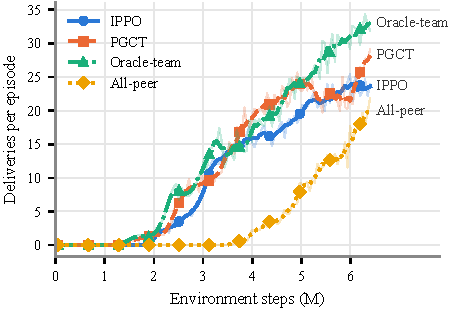
\includegraphics[width=\columnwidth]{figures/fig1_learning_curves.pdf}
\caption{E1의 평가 배송 수/episode(seed 1개\pilot). 가는 선: 51{,}200 step마다의 원 평가값, 굵은 선: 중심 5점 이동평균.}
\label{fig:curves}
\end{figure}

\textbf{주요 비교.} 표~\ref{tab:main}과 그림~\ref{fig:curves}가 E1 비교를 요약한다.\pilot{} \ours{}는 모든 지표에서 독립 학습보다 낫다.
episode당 배송 1개에 0.26M step(13\%) 먼저 도달했고, 학습 중 평균 처리량은 12\%(episode당 11.7 대 10.4), 최종 처리량은 18\%(27.3 대
23.2) 높다. 또한 episode당 배송 20개에 가장 먼저 도달했다(4.15M step, Oracle-team 4.66M, IPPO 5.07M). 팀 라벨 없이 \ours{}는 Oracle-team
평균 처리량의 89\%를 얻는다. 무차별 공유는 초반에 분명히 해롭다. All-peer는 3.99M step에야 episode당 배송 1개에 도달해 다른 방법보다
2백만 step 늦었지만, 실행이 끝날 때 가장 빠르게 오르고 있었다. 이 실행에서는 공유 자체가 아니라 선택성이 차이를 만들었다.

\begin{figure*}[t]
\centering
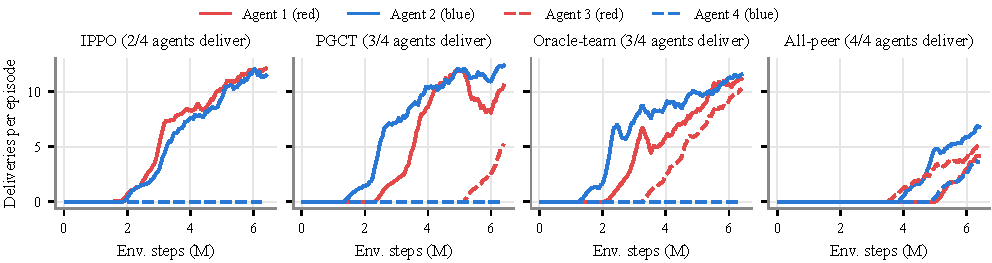
\includegraphics[width=\textwidth]{figures/fig2_per_agent_deliveries.pdf}
\caption{agent별 배송 수/episode(5점 이동평균, seed 1개\pilot). 빨강: 빨강 팀(agent 1, 3), 파랑: 파랑 팀(agent 2, 4). 실선: agent 1--2,
점선: agent 3--4.}
\label{fig:agents}
\end{figure*}

\textbf{선택적 공유는 뒤처진 agent를 돕는다.} agent별 곡선(그림~\ref{fig:agents})이 이득의 출처를 보여 준다. IPPO에서는 팀마다 agent 한 명만
배송을 배웠다. 나머지 두 명은 계속 움직였지만 요청 선반을 한 번도 집지 않았다. 개인 보상이고 팀당 요청이 2개라, 먼저 배운 팀원이 요청 대부분을
처리하고 두 번째 팀원은 배울 만큼의 보상을 받지 못한다. critic distillation은 뒤처진 agent에게 자기 보상 없이도 가치 신호를 준다. \ours{}와
Oracle-team에서는 세 번째 agent가 배웠고(agent 3, 각각 5.4M과 3.6M step부터), All-peer에서는 늦었지만 네 명 모두 배웠다. 배운 agent 한 명이
episode당 약 10--12개를 배송하므로, 학습한 agent 수가 처리량 차이의 대부분을 설명한다. \todo{개입 실험: 뒤처진 agent의 distillation 차단; seed별
학습 agent 수}

\begin{table}[t]
\centering
\small
\resizebox{\columnwidth}{!}{%
\begin{tabular}{lcccc}
\toprule
 & \multicolumn{2}{c}{E1 ($11\times10$)} & \multicolumn{2}{c}{E2 ($16\times16$)} \\
\cmidrule(lr){2-3}\cmidrule(lr){4-5}
방법 & AUC & 마지막 10회 & AUC & 마지막 10회 \\
\midrule
IPPO & 44.57 & 44.52 & 34.24 & 37.61 \\
\ours{} & 45.86 & 46.17 & 34.17 & 37.47 \\
\bottomrule
\end{tabular}}
\caption{공통 커리큘럼 checkpoint에서 4M step 연장 학습(seed 1개\pilot). AUC: 평가 배송 곡선의 정규화 면적, 마지막 10회: 마지막 평가 10회 평균.
이 이전 실험은 학습률 $10^{-4}$, entropy 계수 0.02를 썼다.}
\label{tab:continuation}
\end{table}

\textbf{사전학습 모델에서의 연장.} 공통 사전학습 checkpoint에서 시작하면 \ours{}의 이득은 작다(표~\ref{tab:continuation}). E1에서 AUC +2.9\%,
더 큰 맵에서는 차이가 없다. 이는 위 메커니즘과 맞는다. 모든 agent가 이미 배송할 수 있으면 도울 뒤처진 agent가 없다.

\textbf{팀 목표가 분리된 환경(E1-F).} \todo{E1-F에서 IPPO, All-peer, Oracle-team, \ours{}, \ours{}-v2의 결과, 10M step, seed 1--$n$. 표~\ref{tab:main}과
같은 열에 같은 팀 전이 비율 추가.}
\begin{table}[t]
\centering
\small
\begin{tabular}{lcccc}
\toprule
방법 & 시작 & 평균 & 최종 & 같은 팀 전이 \\
\midrule
IPPO & \tbd & \tbd & \tbd & -- \\
All-peer & \tbd & \tbd & \tbd & \tbd \\
\ours{} & \tbd & \tbd & \tbd & \tbd \\
\ours{}-v2 & \tbd & \tbd & \tbd & \tbd \\
Oracle-team & \tbd & \tbd & \tbd & 100\% \\
\bottomrule
\end{tabular}
\caption{E1-F(팀 목표가 맵 양쪽 모서리). \todo{실행이 끝나면 채움}}
\label{tab:e1f}
\end{table}

\section{분석: gate는 어떤 상대를 고르는가?}
\label{sec:analysis}

\begin{figure*}[t]
\centering
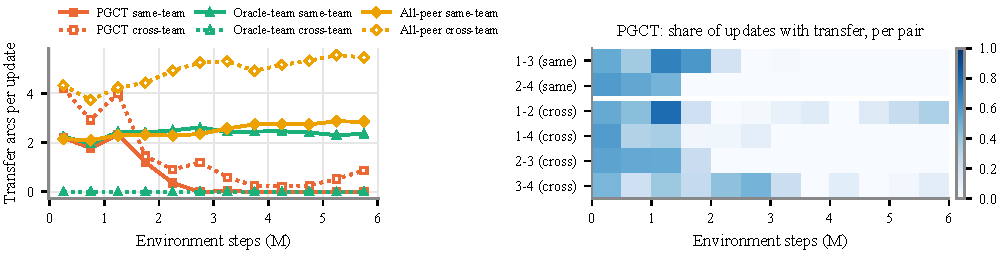
\includegraphics[width=\textwidth]{figures/fig3_critic_transfer.pdf}
\caption{E1의 실제 critic 전이(기록된 할당, warm-up 이후, seed 1개\pilot). 왼쪽: update당 방향성 전이 arc 수, 팀 안(실선)과 팀 간(점선), 0.5M
step 구간 평균. 오른쪽: \ours{}에서 각 agent 쌍이 critic 정보를 주고받은 update 비율.}
\label{fig:transfer}
\end{figure*}

\textbf{학습 중 전이.} 학습 초반에는 모든 정책이 비슷해 gate가 대부분의 이웃을 허용한다(처음 2M step에 update의 91\%에서 전이, 그림~\ref{fig:transfer}).
정책이 분화하면서 gate는 선택적이 된다. 2--4M과 4--6.4M step에서 전이는 update의 37\%와 29\%였고, Oracle-team은 82--86\%, All-peer는 거의 100\%였다.
즉 \ours{}는 두 baseline보다 훨씬 적게 전이하면서 All-peer보다 빨리 학습했다. \emph{어떤} critic을 distillation하느냐가 얼마나 많이 하느냐보다 중요함을
시사한다.

\textbf{상대는 팀원이 아니라 호환되는 agent다.} E1에서 gate의 후반 연결은 주로 팀 간이었다(agent 3--4, 이후 1--2; 4M step 이후 update당 같은 팀
0.03 arc, 다른 팀 0.63 arc). 이는 이 환경에서 선택의 실패가 아니다. 관측이 팀 기준이고 두 목표가 붙어 있어 두 팀은 같은 결정 문제를 푼다. agent 사이에
다른 것은 역할(자기 구역에 머무는가, 상대 구역에서 선반을 가져오는가)과 숙련도다. 별도의 고정 정책 평가에서, 팀원의 critic은 실제로 팀원이 아닌
agent의 critic보다 \emph{덜} 호환됐다. receiver의 critic을 팀원의 critic과 섞었을 때 가치 오차가 줄어든 정도가 팀원이 아닌 agent와 섞었을 때보다
작았다(E1 checkpoint 4개에서 같은 팀 AUROC 0.25--0.33). 따라서 gate는 행동이, 그리고 실측상 가치 예측도 호환되는 상대를 고르며, 팀 대칭 과제에서는
그것이 팀을 가로지른다. 팀의 목표가 실제로 다를 때 gate가 팀을 찾는지는 E1-F에서 다룬다. \todo{E1-F gate 분석}

\begin{figure}[t]
\centering
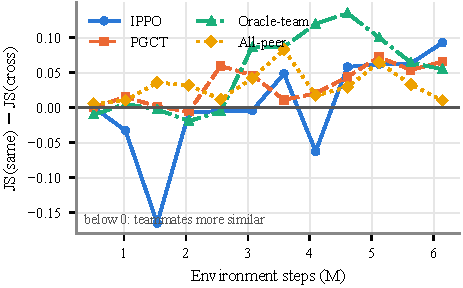
\includegraphics[width=\columnwidth]{figures/fig4_probe_js_gap.pdf}
\caption{E1 checkpoint에서 팀원 사이 probe 거리에서 팀원이 아닌 쌍의 probe 거리를 뺀 값(seed 1개\pilot). 0보다 크면 팀원의 정책이 더 다르다.}
\label{fig:jsgap}
\end{figure}

\textbf{probe 집합의 팀 정보.} 2.5M step 이후 거의 모든 checkpoint에서, 모든 방법의 팀원 사이 probe 거리가 팀원이 아닌 쌍보다 컸다(그림~\ref{fig:jsgap}).
팀과 무관한 probe 집합은 agent의 팀 기준 관점에서 목표가 똑같아 보이는 팀들을 구분할 수 없다. 그래서 v2 집합에는 목표가 보이지 않는 상태에서 선반을
든 probe를 넣었다. 이 상황에서는 팀이 학습한 목표 위치가 행동을 정한다. \todo{E1-F에서 v2 gate의 팀 구분}

\section{논의와 한계}
\textbf{예비 증거.} E1의 모든 수치는 training seed 1개에서 나왔다. 같은 seed와 같은 가중치로 다시 실행하면 IPPO는 정확히 재현됐지만 공유 방식들은
1.4--1.6M step 이후 갈라졌다(부록 B). 그 재실행에서 All-peer의 배송 시작 시점은 2백만 step 차이가 났다. 따라서 비교에는 여러 seed가 필요하며, 현재
실행 중이다. \todo{평균과 95\% 구간 보고; 비결정적 연산 확인}

\textbf{가정.} \ours{}는 공유 probe 집합, 모델 출력의 국소 통신, 같은 probe가 모든 agent에게 같은 의미를 갖는 관측 공간을 가정한다. 우리 환경에서
probe 집합은 맵 배치에서 고정 규칙으로 생성한다. 환경에 무관한 자동 probe 생성은 향후 과제다.

\textbf{범위.} agent 4명, 팀 2개의 한 환경 계열을 평가했다. 더 많은 agent와 팀, 팀 공유 보상, 중앙 baseline(MAPPO, SePS 방식, HetDPS 방식 공유)과의
비교는 계획되어 있다. \todo{baseline}

\section{결론}
우리는 각 agent가 공유 probe 집합에 대한 모델 출력으로 누구의 critic에서 배울지 정하는 분산 방법 \ours{}를 제안했다. 두 팀 창고 과제의 예비 실험에서
선택적 critic 공유는 독립 학습과 무차별 공유를 모두 앞섰고 정답 팀원과의 공유에 근접했다. 이 이득은 주로 뒤처진 agent가 학습하게 한 데서 나왔다. 두
팀이 같은 문제를 푸는 과제에서 gate는 팀원이 아니라 호환되는 상대를 골랐다. 팀 목표가 갈라지는 실험과 더 많은 seed로, 정책 유사도에 의한 상대 선택이
언제 팀 소속과 일치하는지 확인할 것이다.

\bibliographystyle{plainnat}
\bibliography{references}

\clearpage
\appendix
\onecolumn

\section{하이퍼파라미터}
\begin{table}[h]
\centering
\small
\begin{tabular}{ll}
\toprule
Setting & Value \\
\midrule
Map / agents / teams & 11$\times$10 E1 / 4 / 2 \\
Reward & individual \\
Home-zone shelf ratio & 0.5 \\
Requests per team & 2 \\
Sensor / communication range & 5 / 5 \\
Learning rate & 0.0002 \\
Entropy coef. & 0.05 \\
$\gamma$ / GAE $\lambda$ & 0.99 / 0.95 \\
Rollout / BPTT length & 1024 / 64 \\
PPO epochs / minibatches / clip & 4 / 8 / 0.2 \\
Hidden (MLP / GRU) & 128 / 128 \\
Peer-loss coef. $\lambda_{peer}$ & 0.01 \\
Gate: JS threshold / EMA $\beta$ / warm-up & 0.12 / 0.35 / 100 upd. \\
Canonical probes & 48 (fixed, zero hidden, length 1) \\
Evaluation & every 50 updates, 20$\times$500 steps, deterministic \\
\bottomrule
\end{tabular}

\caption{처음부터 학습한 E1 비교의 설정(donor 집합을 제외하고 모든 방법이 동일).}
\end{table}

\section{같은 seed에서의 재현성}
\begin{figure}[h]
\centering
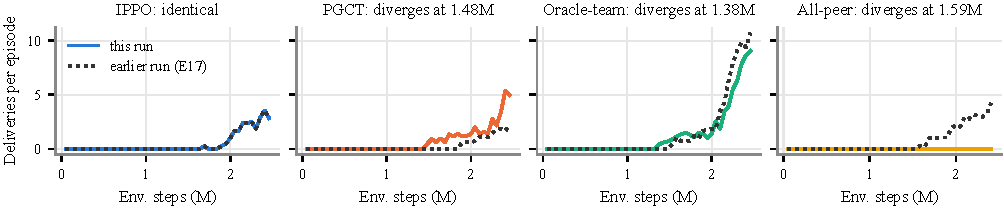
\includegraphics[width=\textwidth]{figures/figA1_reproducibility.pdf}
\caption{같은 seed와 초기 가중치의 두 실행(실선: 보고한 실행, 점선: 이전에 중단된 실행). IPPO는 정확히 재현되고, 공유 방식은 1.4--1.6M step 이후 갈라진다.}
\end{figure}

\section{구간별 실제 전이}
\begin{table}[h]
\centering
\small
\begin{tabular}{llccc}
\toprule
Method & Window & Updates w/ transfer & Same-team arcs/upd. & Cross-team arcs/upd. \\
\midrule
PGCT & 0--2.0M & 91\% & 1.86 & 3.09 \\
 & 2--4.0M & 37\% & 0.10 & 0.73 \\
 & 4--6.4M & 29\% & 0.03 & 0.63 \\
\addlinespace
Oracle-team & 0--2.0M & 82\% & 2.26 & 0.00 \\
 & 2--4.0M & 86\% & 2.50 & 0.00 \\
 & 4--6.4M & 85\% & 2.39 & 0.00 \\
\addlinespace
All-peer & 0--2.0M & 99\% & 2.22 & 4.18 \\
 & 2--4.0M & 100\% & 2.49 & 5.10 \\
 & 4--6.4M & 100\% & 2.79 & 5.37 \\
\bottomrule
\end{tabular}

\caption{E1의 학습 구간별 실제 전이(seed 1개). arc는 receiver--donor 방향 연결이다.}
\end{table}

\section{커리큘럼 모델의 역할}
\begin{figure}[h]
\centering
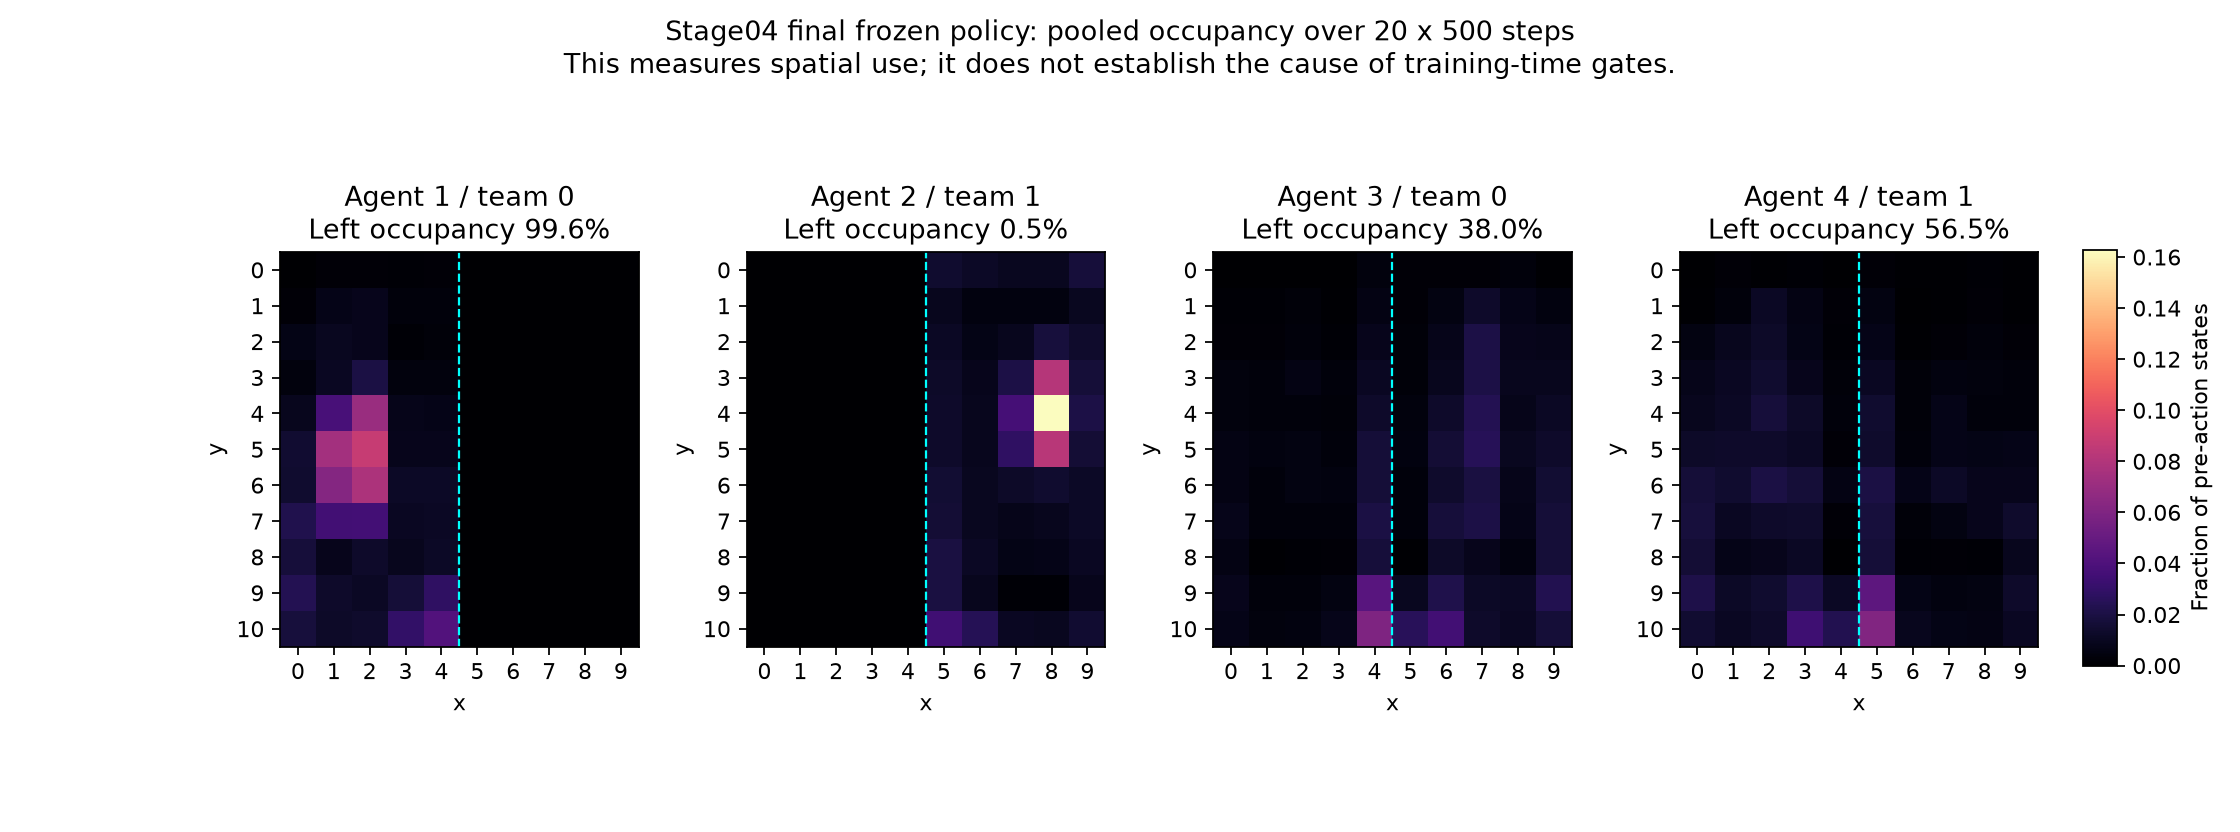
\includegraphics[width=\textwidth]{figures/stage04_occupancy.png}
\caption{선반의 50\%를 상대 팀 구역에 둔 고정 커리큘럼 모델의 칸 점유(20$\times$500 step). agent 1과 2는 자기 팀 구역에 머물고, agent 3과 4는 상대 구역에서
선반을 가져오며 gate가 가장 자주 연결한 쌍이다.}
\end{figure}

\end{document}
